\documentclass[color=usenames,dvipsnames]{beamer}\usepackage[]{graphicx}\usepackage[]{color}
% maxwidth is the original width if it is less than linewidth
% otherwise use linewidth (to make sure the graphics do not exceed the margin)
\makeatletter
\def\maxwidth{ %
  \ifdim\Gin@nat@width>\linewidth
    \linewidth
  \else
    \Gin@nat@width
  \fi
}
\makeatother

\definecolor{fgcolor}{rgb}{0.345, 0.345, 0.345}
\newcommand{\hlnum}[1]{\textcolor[rgb]{0.686,0.059,0.569}{#1}}%
\newcommand{\hlstr}[1]{\textcolor[rgb]{0.192,0.494,0.8}{#1}}%
\newcommand{\hlcom}[1]{\textcolor[rgb]{0.678,0.584,0.686}{\textit{#1}}}%
\newcommand{\hlopt}[1]{\textcolor[rgb]{0,0,0}{#1}}%
\newcommand{\hlstd}[1]{\textcolor[rgb]{0.345,0.345,0.345}{#1}}%
\newcommand{\hlkwa}[1]{\textcolor[rgb]{0.161,0.373,0.58}{\textbf{#1}}}%
\newcommand{\hlkwb}[1]{\textcolor[rgb]{0.69,0.353,0.396}{#1}}%
\newcommand{\hlkwc}[1]{\textcolor[rgb]{0.333,0.667,0.333}{#1}}%
\newcommand{\hlkwd}[1]{\textcolor[rgb]{0.737,0.353,0.396}{\textbf{#1}}}%
\let\hlipl\hlkwb

\usepackage{framed}
\makeatletter
\newenvironment{kframe}{%
 \def\at@end@of@kframe{}%
 \ifinner\ifhmode%
  \def\at@end@of@kframe{\end{minipage}}%
  \begin{minipage}{\columnwidth}%
 \fi\fi%
 \def\FrameCommand##1{\hskip\@totalleftmargin \hskip-\fboxsep
 \colorbox{shadecolor}{##1}\hskip-\fboxsep
     % There is no \\@totalrightmargin, so:
     \hskip-\linewidth \hskip-\@totalleftmargin \hskip\columnwidth}%
 \MakeFramed {\advance\hsize-\width
   \@totalleftmargin\z@ \linewidth\hsize
   \@setminipage}}%
 {\par\unskip\endMakeFramed%
 \at@end@of@kframe}
\makeatother

\definecolor{shadecolor}{rgb}{.97, .97, .97}
\definecolor{messagecolor}{rgb}{0, 0, 0}
\definecolor{warningcolor}{rgb}{1, 0, 1}
\definecolor{errorcolor}{rgb}{1, 0, 0}
\newenvironment{knitrout}{}{} % an empty environment to be redefined in TeX

\usepackage{alltt}
%\documentclass[color=usenames,dvipsnames,handout]{beamer}

%\usepackage[roman]{../pres1}
\usepackage[sans]{../pres1}




\IfFileExists{upquote.sty}{\usepackage{upquote}}{}
\begin{document}



\begin{frame}[plain]
  \begin{center}
    {\huge \bf Mark-recapture methods for estimating survival and recruitment \par}
%    \vspace{0.5cm}
%    { \Large April 8 \& 10, 2019} \\
    {\color{blue} \rule{\textwidth}{1pt}}
    \vfill
    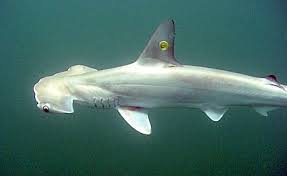
\includegraphics[height=3cm,keepaspectratio]{figs/hammerhead} %\hfill
    \hspace{0.5cm}
    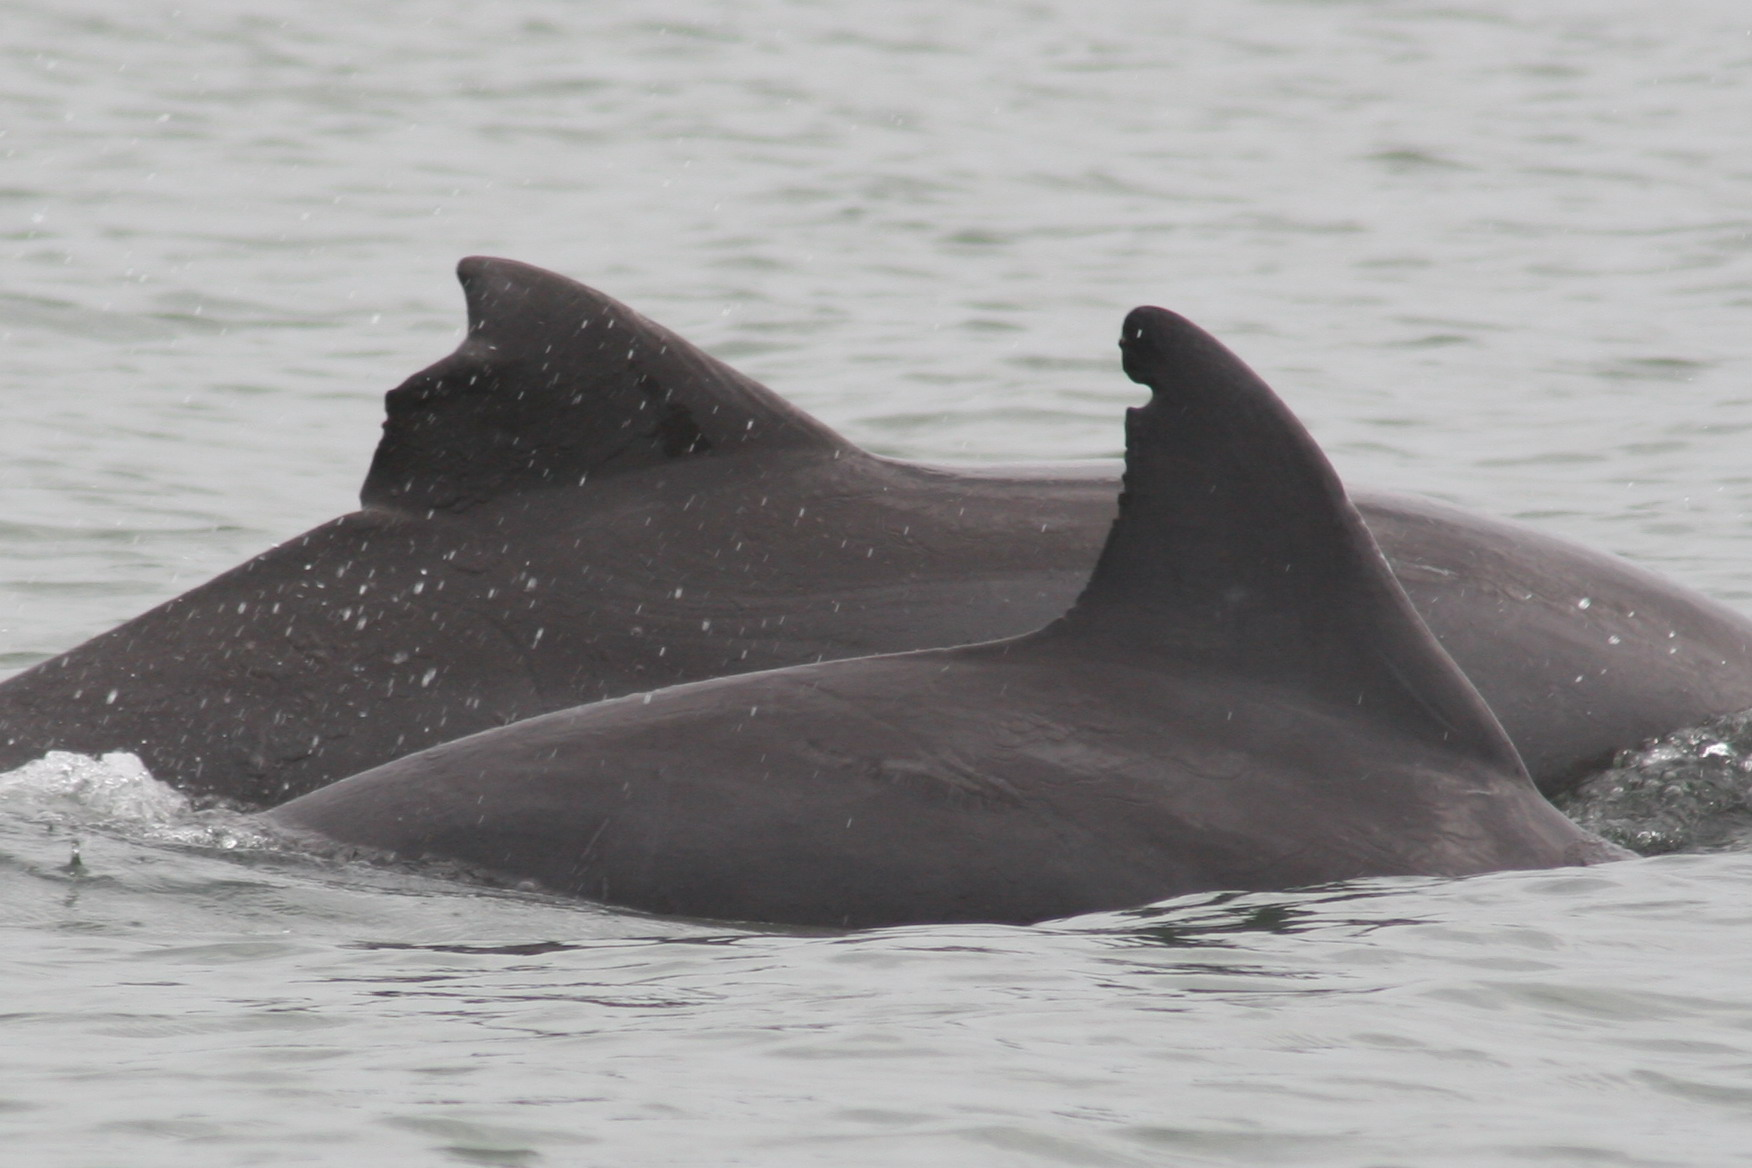
\includegraphics[height=3cm,keepaspectratio]{figs/dolphins}
  \end{center}
\end{frame}





\section{Introduction}






\begin{frame}
  \frametitle{Outline}
  \Large
  \tableofcontents[hideallsubsections]
%  \only<1>{\tableofcontents[hideallsubsections]}
%  \only<2>{\tableofcontents[currentsection,hideallsubsections]}
\end{frame}





\begin{frame}
  \frametitle{Accounting for imperfect detection}
%  \large
%  \bf
  Suppose we mark and { release} $R$ individuals, and then
    recapture $m$ of them on the second occasion. \par
%    \vspace{0.5cm}
    \vfill
    \uncover<2->{
      How do we estimate survival probability? \par
      }
%    \vspace{0.5cm}
    \vfill
    \uncover<3->{
      If capture probability ($p$) was 1, we could use:
      \[ %\Large
        \hat{S} = \frac{m}{R}
      \]}
    \vspace{-12pt}
    \uncover<4->{ \flushleft
      But when $p<1$, $m$ is some fraction of the number actually
      alive ($M$), so we have to estimate $p$ and $M$ to estimate $S$: %\par
      }
    \vfill
  \begin{columns}
    \begin{column}<5->{.333\textheight}
      \[ %\Large
      \hat{S} = \frac{\hat{M}}{R}
      \]
    \end{column}
    \begin{column}<6->{.333\textheight}
      \centering where \par
    \end{column}
    \begin{column}<7->{.333\textheight}
      \[ %\Large
      \hat{M} = \frac{m}{\hat{p}}
      \]
    \end{column}
  \end{columns}
%  \vfill
%  \uncover<8>{ \centering
%  The challenge is estimating $p$ \\
%  }
%   \begin{itemize}
%     \item $N$ is abundance (population size)
% %      \footnote{Density is just $\hat{D} = \hat{N}/A$}
%     \item $n$ is the number of individuals detected
%     \item $\hat{p}$ is an estimate of detection probability: The probability
%       of detecting an individual.
%   \end{itemize}
%   \pause
%   \vfill
%   \Large \bf
%   Most methods differ in how they estimate $p$
\end{frame}









\section{Tag recovery models}


\begin{frame}
  \frametitle{Tag recovery models}
%  \large
  {\bf Purpose} \\
  Estimate survival from recovered tags \\
  \vspace{0.5cm}
  \begin{center}
    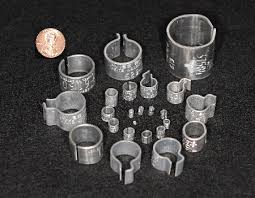
\includegraphics[height=3.5cm,keepaspectratio]{figs/metal-bands}
    % \hfill
    \hspace{0.5cm}
    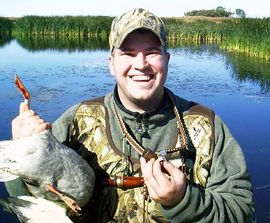
\includegraphics[height=3.5cm,keepaspectratio]{figs/duck-hunter}
  \end{center}
  \pause
  {\bf Benefit} \\
  Because hunters are just about everywhere, we don't have to worry
  about animals leaving `the study area' and we can estimate actual
  survival.
\end{frame}



\begin{frame}
  \frametitle{Tag recovery models}
  {\bf Design}
  \begin{itemize}
    \item Animals are marked and released
    \item Hunters or anglers report tags from harvested individuals
    \item Desirable to have at least 5 releases
  \end{itemize}
  \pause
%  \vspace{0.5cm}
  \vfill
  {\bf Data}                                                 \\
  Two release years followed by 2 years of recoveries:
  \begin{center}
    \begin{tabular}{ccc}
      \hline
      Number released & \multicolumn{2}{c}{Period recovered} \\
      \cline{2-3}
                      & 1         & 2                        \\
      \hline
      $R_1$           & $m_{1,1}$ & $m_{1,2}$                \\
      $R_2$           &           & $m_{2,2}$                \\
      \hline
    \end{tabular}
  \end{center}
  \pause
  \vfill
  {\bf Parameters}                                           \\
  \begin{itemize}
    \item Survival ($S$)
    \item Recovery rate ($f$)
  \end{itemize}
\end{frame}


\begin{frame}
  \frametitle{Tag recovery models}
  {\bf Expected values}
  \begin{center}
    \begin{tabular}{lcccc}
      \hline
      Period released & Number released & \multicolumn{3}{c}{Period recovered} \\
      \cline{3-5}
                    &  & 1 & 2 & 3 \\
      \hline
      1 & $R_1$ & $R_1f_1$ & $R_1S_1f_2$ & $R_1S_1S_2f_3$ \\
      2 & $R_2$ &          & $R_2f_2$ & $R_2S_2f_3$ \\
      3 & $R_3$ &          &          & $R_3f_3$ \\
      \hline
    \end{tabular}
  \end{center}
  \pause
  \vfill
  \centering
  Software programs like {\tt MARK} find the most likely values of $S$
  and $f$, given the data. \\
\end{frame}




\begin{frame}
  \frametitle{Tag recovery models}
  \large
  {\bf Assumptions}
  \begin{itemize}
    \item Sample is representative of population
    \item No tag loss, mis-identification, etc\dots
    \item All animals have common survival and recovery rates
    \item Fates are independent
  \end{itemize}
  \pause
  \vspace{0.5cm}
  {\bf Extensions}
  \begin{itemize}
    \item Age-specific models
    \item Grouping variables
    \item Time variables
    \item Habitat variables
  \end{itemize}
\end{frame}




\section{CJS model}

\begin{frame}
  \frametitle{Cormack-Jolly-Seber (CJS) model}
  {\bf Purpose} \\
  Estimate survival and capture probability from capture-recapture data \\
  \pause
  \vspace{0.5cm}
  {\bf Design} \\
  A random sample of animals is marked and followed over many periods
  (usually years) \\
%  {\bf Examples}
%  \begin{itemize}
%    \item Target-netting birds
%  \end{itemize}
  \pause
  \vspace{0.5cm}
  {\bf Notes} \\
  \begin{itemize}[<+->]
    \item When permanent emigration is possible, we can't be sure if
    an animal died or left study area
    \item So, we often have to estimate ``apparent survival'' ($\phi$)
      instead of actual survival ($S$)
    \item Apparent survival is the probability that an individual
      survives and does not permanently emigrate out of the study area
  \end{itemize}
\end{frame}


% \begin{frame}
%   \frametitle{CJS in spanish}
%   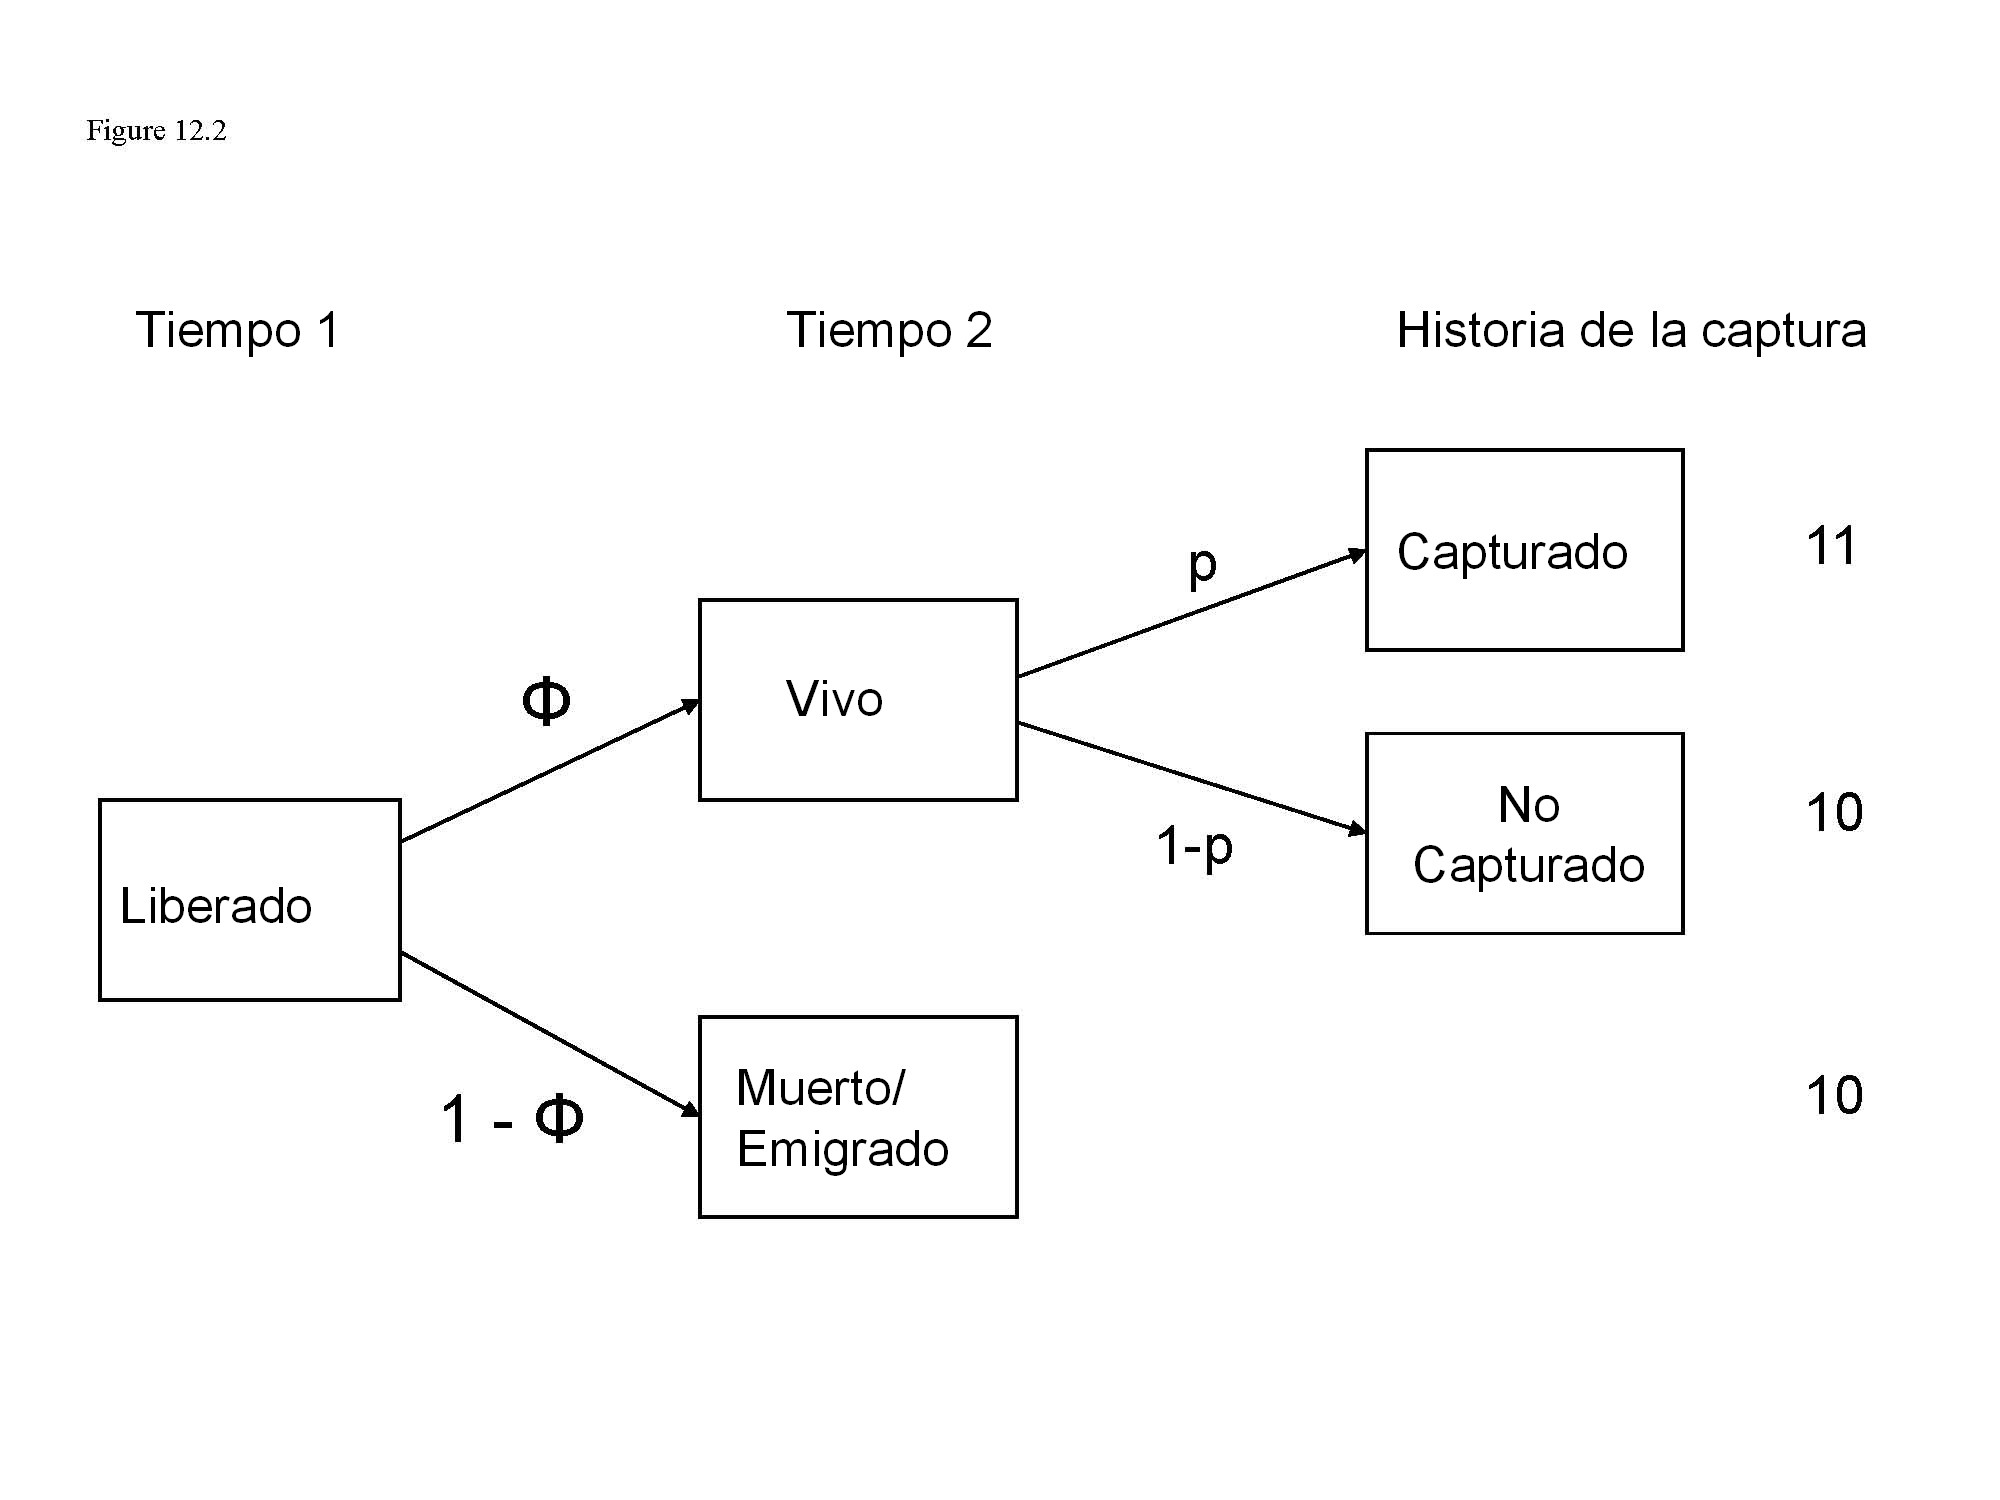
\includegraphics[width=\textwidth]{figs/CJS}
% \end{frame}



\begin{frame}
  \frametitle{CJS capture histories}
%  {\bf Animals are marked and followed over may periods (usually
%    years) \par}
%  \pause
%  \vspace{0.3cm}
  In CJS studies, we ignore the leading zeros in the capture histories
  because we aren't interested in how animals enter the sample \\
  \vfill
  \uncover<2->{All we care about is survival, so we ``condition'' on first encounter \\}
%  {\bf \centering \large $n=5$ individuals captured over 3 sampling occasions \par}
%  \vspace{0.3cm}
  \vfill
  \begin{center}
    \small
    \begin{tabular}{lccc}
      \hline
      & Year 1 & Year 2 & Year 3 \\
      \hline
      Animal 1 & 1 & 0 & 0 \\
      Animal 2 &  & 1 & 0 \\
      Animal 3 &  &  & 1 \\
      Animal 4 & 1 & 1 & 1 \\
      Animal 5 &  & 1 & 1 \\
      \hline
    \end{tabular}
  \end{center}
\end{frame}



\begin{frame}
  \frametitle{CJS capture histories}
  \large
  Estimation is accomplished by finding the values of $p$ and $\phi$
  that best align the expected values with the observed capture
  histories \\
  \vfill
  \begin{center}
    \begin{tabular}{ll}
      \hline
      Capture history & Expected values \\
      \hline
      111 & $\phi_1p_2\phi_2p_3$ \\ %\pause
      110 & $\phi_1p_2(1-\phi_2p_3)$ \\ %\pause
      101 & $\phi_1(1-p_2)\phi_2p_3$ \\ %\pause
      100 & $(1-\phi_1)+\phi_1(1-p_2)(1-\phi_2p_3)$ \\
      \hline
    \end{tabular}
  \end{center}
%  The observed capture histories allow us to estimate the parameters
\end{frame}





\begin{frame}
  \frametitle{CJS model}
  {\bf Assumptions}
  \begin{itemize}
    \item Same as tag-recovery, plus\dots
    \item Instantaneous recapture and release of animals
    \item Homogeneity of capture and survival probabilities for marked
      animals
    \item All emigration is permanent
  \end{itemize}
  \pause
  \vspace{0.5cm}
  {\bf Model can be extended to accommodate variation due to\dots}
  \begin{itemize}
    \item Age
    \item Sex
    \item Habitat
    \item Geographical regions
  \end{itemize}

\end{frame}


\section{JS model}


\begin{frame}
  \frametitle{Jolly-Seber (JS) model}
  {\bf Purpose} \\
  Estimate survival, recruitment, abundance, and capture probability
  from capture-recapture data \\
  \pause
  \vspace{0.5cm}
  {\bf Design} \\
  Randomly sample the population during every period and mark all
  newly captured unmarked animals \\
  \pause
  \vspace{0.5cm}
  {\bf Examples}
  \begin{itemize}
    \item Constant-effort mist-netting
    \item Long-term small mammal trapping
  \end{itemize}
\end{frame}



\begin{frame}
  \frametitle{JS capture histories}
%  {\bf \centering \large $n=5$ individuals captured over 3 sampling occasions \par}
%  \vspace{0.3cm}
  {We no longer ``condition'' on first encounter -- Instead, we use
    all the data. \\}
  \vfill
  The leading zeros provide information about when individuals are
  recruited into the population \\
  \vfill
  \begin{center}
    \small
    \begin{tabular}{lccc}
      \hline
      & Year 1 & Year 2 & Year 3 \\
      \hline
      Animal 1 & 1 & 0 & 0 \\
      Animal 2 & 0 & 1 & 0 \\
      Animal 3 & 0 & 1 & 1 \\
      Animal 4 & 1 & 1 & 1 \\
      Animal 5 & 0 & 1 & 1 \\
      \hline
    \end{tabular}
  \end{center}
\end{frame}



\begin{frame}
  \frametitle{Jolly-Seber model}
  {\bf Assumptions}
  \begin{itemize}
    \item All the assumptions of CJS model, plus\dots
    \item Every animal --- marked or unmarked --- has the same
      probability of capture
  \end{itemize}
  \pause
  \vfill
  The standard JS model doesn't work very well, but it is extremely
  powerful when combined with \emph{the robust design}.
\end{frame}



\section{Robust design}



% \begin{frame}
%   \frametitle{Robust design}
%   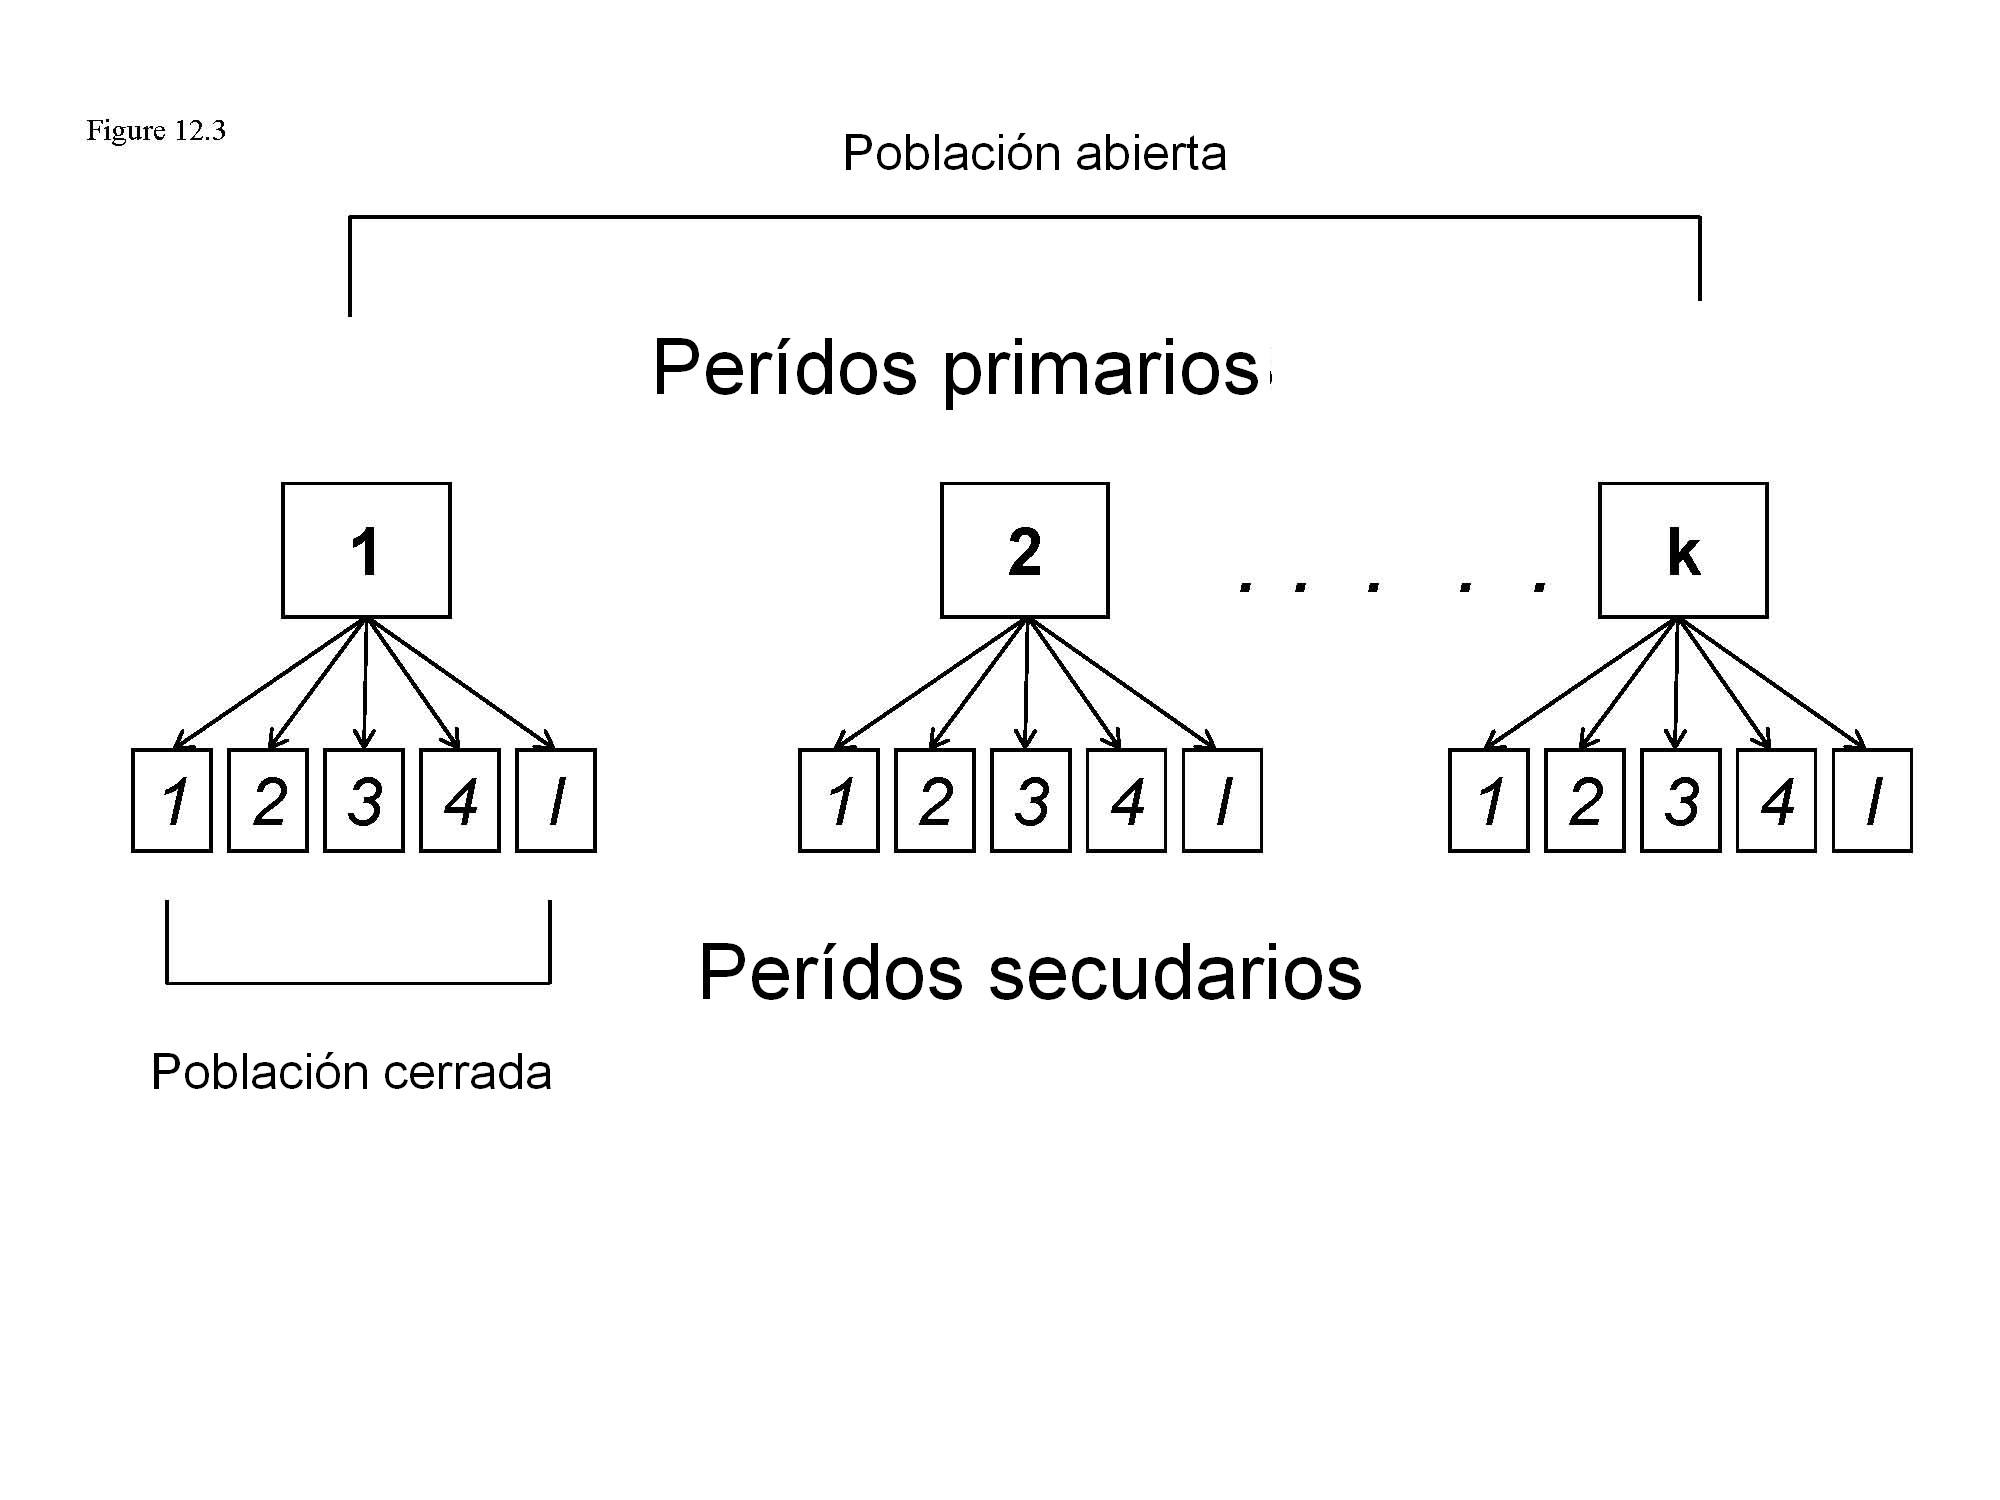
\includegraphics[width=\textwidth]{figs/robust-design}
% \end{frame}



\begin{frame}
  \frametitle{Robust design}
%  \large
  {\bf Purpose} \\
  Relax assumptions and increase precision by collecting more data \\
  \pause
  \vspace{0.5cm}
  {\bf Key concept} \\
  We now have two types of sampling periods:
  \begin{enumerate}[<+- | visible@+->][\bf \color{PineGreen} (1)]
    \item \alert{Primary sampling periods} between which the population
      is assumed to be demographically open
    \item \alert{Secondary sampling periods} over which the population
      is assumed closed
  \end{enumerate}
  \uncover<4>{
  \vfill
  The replicate surveys with each primary period give us direct
  information about capture probability, which makes it easier to
  estimate the other parameters.
  }
\end{frame}


\begin{frame}
  \frametitle{Robust design capture histories}
%  \begin{center}
  \centering %\\
%    \tiny
    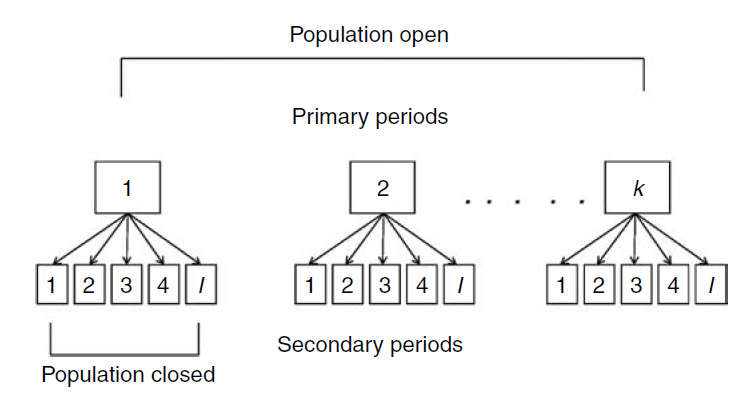
\includegraphics[width=0.65\textwidth]{figs/robustDesign} \\
  \vfill
  \pause
  Example with 2 primary periods and 3 secondary periods \\
%    \centering
  \small
    \begin{tabular}{lccccccc}
%      \small
      \hline
      & \multicolumn{3}{c}{Primary period 1} & &
        \multicolumn{3}{c}{Primary period 2} \\
      \cline{2-4} \cline{6-8}
      & Day 1 & Day 2 & Day 3 & & Day 1 & Day 2 & Day 3 \\
      \hline
      Animal 1 & 0 & 0 & 1 & & 1 & 0 & 0 \\
      Animal 2 & 0 & 0 & 0 & & 0 & 0 & 0 \\
      Animal 3 & 0 & 0 & 0 & & 1 & 0 & 0 \\
      Animal 4 & 1 & 1 & 1 & & 0 & 0 & 0 \\
      Animal 5 & 0 & 0 & 0 & & 1 & 1 & 0 \\
      \hline
    \end{tabular}
%  \end{center}
\end{frame}





\begin{frame}
  \frametitle{Summary}
  \begin{tabular}{lllll}
    \hline
    Method & Data & Survival & Recruitment & Abundance \\
    \hline
    Tag recovery & Recoveries & Yes & No & No \\
    CJS & Mark-recap & Yes\footnote{Apparent survival} & No & No \\
    JS & Mark-recap & Yes$^1$ & Yes & Yes \\
    \hline
  \end{tabular}
  \vfill
  \centering
  Each of these three methods is widely used in practice. The best
  option depends on the objectives \\.
%  \vfill
%  $^*$ Apparent survival
\end{frame}


% \begin{frame}
%   \frametitle{Summary}
%   \large
%   \begin{itemize}
%     \item Capture-recapture methods use information about recapture
%       rates to estimate capture probability and abundance
%     \item More advanced methods can be used to estimate density and
%       vital rates
%     \item Modern field methods use camera traps or DNA sampling
%       techniques to collect non-invasive capture-recapture data
%   \end{itemize}
% \end{frame}



\end{document}


